\documentclass[conference]{IEEEtran}
% ISCAS 2027: IEEEtran conference mode, US letter, 4 pages of content + 1 optional page of references only.
\IEEEoverridecommandlockouts
\usepackage{cite}
\usepackage{amsmath}
\usepackage{newtxtext,newtxmath}
\usepackage{graphicx}
\usepackage{booktabs}
\usepackage{siunitx}
\usepackage[hidelinks]{hyperref}
\sisetup{detect-all, per-mode=symbol}
\graphicspath{{../figs/}}
\newcommand{\Vg}{V_\mathrm{gate}}
\newcommand{\Vd}{V_\mathrm{drain}}
\newcommand{\Vdel}{V_\mathrm{DEL}}

\begin{document}

\title{A Post-Fabrication-Tunable Time-Domain Multi-Row Read for RRAM Processing-in-Memory}

\author{\IEEEauthorblockN{Eyal Yemini, Adam Teman, and Leonid Yavits}
\IEEEauthorblockA{Faculty of Engineering, Bar-Ilan University, Ramat Gan, Israel\\
eyal.yemini@live.biu.ac.il}}

\maketitle

\begin{abstract}
Resistive RAM (RRAM) turns a memory array into a computing element, because a read that opens several rows sums the conductances of the selected cells on the bit line.
The circuit that resolves this sum is designed against a device model, yet the model captures neither the resistance spread of a programmed array nor the capacitance of the memory stack, so a read designed for one operating point can miss the point at which the fabricated cells sit.
This paper presents a read path whose operating point is chosen after fabrication.
Each column converts the bit-line discharge time into a thermometer code, and the sampling window, tap pitch, and drive levels are set from registers and supply pads, so that opening several rows turns a read into an in-memory NOR or majority without a reference cell.
In a tape-out-ready 64$\times$64 one-transistor-one-resistor macro, post-layout simulation resolves a single row by all eight taps, an 8-row NOR by six, and an 8-row majority by two, at 1.0 to 1.7\,pJ per 64-bit result, and a Monte Carlo analysis converts these margins into the resistance spread the device has to meet, 0.45 in $\ln R$ for a single row and 0.17 for eight.
\end{abstract}

\begin{IEEEkeywords}
RRAM, 1T1R, processing-in-memory, time-domain readout, time-to-digital converter.
\end{IEEEkeywords}

\section{Introduction}
\label{sec:intro}
Resistive RAM (RRAM) in a one-transistor-one-resistor (1T1R) array stores data as conductance.
When several word lines open at once, the bit line sums the conductances of the selected cells,
and the array becomes a computing element. A multi-row read then yields bulk bitwise
operations~\cite{li2016pinatubo} or an analog multiply-accumulate~\cite{chi2016prime,shafiee2016isaac}
in a single access~\cite{ielmini2018inmemory}. Stateful memristive logic complements this by writing
the result into a cell: material implication~\cite{borghetti2010memristive}, NOR~\cite{kvatinsky2014magic},
majority~\cite{gaillardon2016plim}.
Silicon demonstrations of RRAM processing-in-memory (PiM) rely on dedicated sense circuits with
tracking references or calibration~\cite{chen2018rram65nm,wan2022neurram}, and time-domain readout with TDCs digitizes
in-memory multiply-accumulate compactly~\cite{sayal2020timedomain,xue2024tdcim}. On an academic research chip, however, the operating point of the memory element is known only
after tape-out, and so are its resistance spread and its parasitic capacitances. The readout
therefore has to be \emph{tunable after fabrication}, not optimized for one assumed point.

This paper presents a PiM read path designed for that situation, verified to a tape-out-ready
64$\times$64 macro in the IHP SG13G2 130\,nm BiCMOS process with its back-end HfAlO RRAM
module~\cite{perez2017hfalo}. Instead of voltage-mode sense
amplifiers, every column converts the bit-line \emph{discharge time} into an 8-bit thermometer
code with an 8-tap delay-line TDC. With several rows open the discharge time measures the summed cell conductance, i.e.\ an
in-memory NOR or majority. The sampling instant, tap pitch and drive levels are all set from
software, through dedicated supply pads and a register-programmable controller. Unlike the reference-tracked or calibrated sense circuits of~\cite{chen2018rram65nm,wan2022neurram}
and the MAC-oriented TDC readouts of~\cite{sayal2020timedomain,xue2024tdcim}, this is a
bitwise-logic read whose decision window is placed after fabrication. All results are pre-silicon.

The contributions are: (i) a time-domain multi-row read whose window position, tap pitch and
drive levels are set after fabrication by a 21-state controller, co-verified in SPICE/AMS with
the RTL (Sections~\ref{sec:macro}, \ref{sec:ctrl}); (ii) a transistor-level evaluation of NOR
and majority as decision margins in TDC taps over the read supplies, the state resistance and
the number of rows, with energy and read disturb (Section~\ref{sec:results}); and (iii) a
budget derived from those margins: the resistance spread, corners and temperatures each
operation tolerates, i.e.\ what the RRAM cell has to provide for the read to work.

\section{Post-Fabrication-Tunable Time-Domain Read}
\label{sec:read}
\begin{figure}[!t]
\centering
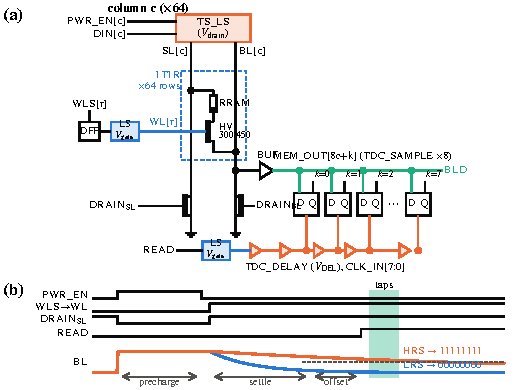
\includegraphics[width=\columnwidth]{schematic}
\caption{(a) One column of the macro with its TDC. (b) Read sequence, with the eight-tap window shaded.}
\label{fig:schematic}
\end{figure}
If the model cannot say where the fabricated cells will sit, the read circuit has to be able to find them, and this section proposes a read built around that requirement.
Fig.~\ref{fig:schematic} shows the proposed post-fabrication-tunable time-domain readout circuit and its read sequence.
A conventional sense amplifier asks whether the bit line is above or below a reference at one instant, whereas this read asks how long the bit line takes to discharge.
A read precharges the bit line BL to the drive voltage $\Vd$, opens the selected rows, and then grounds the source line SL, so that BL discharges through the selected cells with a time constant set by the cell resistance, the access-transistor resistance, and the bit-line capacitance.
A buffer with a threshold of about 0.6\,V converts BL into a digital signal, and eight flip-flops sample this signal on the eight taps of a delay line that a READ pulse triggers.
The result is a thermometer code that counts the taps at which BL was still high, so that a low-resistance (LRS) cell gives a short code and a high-resistance (HRS) cell a long one (Fig.~\ref{fig:schematic}(b)).

Three knobs place the decision, and none of them is a transistor size.
The controller inserts a signed offset between the grounding of SL and the READ pulse in 10\,ns steps, which moves the sampling window along the discharge; a dedicated supply pad $\Vdel$ sets the delay of the line and with it the tap pitch; and the word-line supply $\Vg$ sets the access-transistor resistance together with the level-shifter delay.
All three are registers or pads, so the window can be placed after the resistance and the capacitance of the fabricated cells have been measured, and no reference cell has to be programmed with the same uncertain device.

With $n$ rows open, the column conductance is the sum of the selected cells, so the discharge time, and with it the code $c(k)$, falls monotonically with the number $k$ of LRS cells among them.
The in-memory operations are thresholds on this code, each with a margin measured in taps.
A NOR over the $n$ rows separates $k=0$ from $k\ge1$ with a margin of $c(0)-c(1)$, and a majority separates $k\le n/2$ from $k>n/2$ with a margin of $c(n/2)-c(n/2+1)$.
These bitwise operations over an arbitrary row mask are the primitive of digital PiM~\cite{li2016pinatubo}, and here they come out of the same read that serves a single row.

\section{Macro and Controller}
\label{sec:impl}
\begin{figure}[!t]
\centering
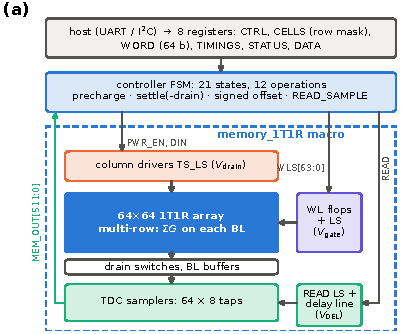
\includegraphics[height=1.4in]{macro_arch}\hfill
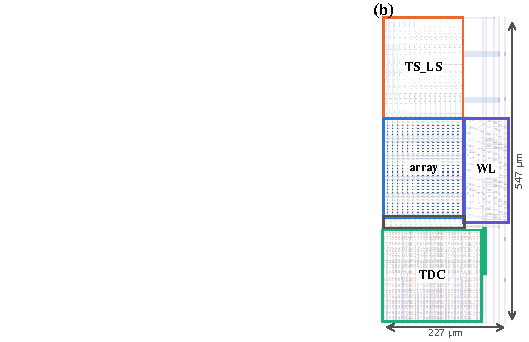
\includegraphics[height=1.4in]{macro_layout_crop}
\caption{(a) Macro and controller architecture. (b) Tape-out-ready layout, 226.5$\times$547.4\,\si{\micro\meter}.}
\label{fig:macro}
\end{figure}
The read path is implemented in a 64$\times$64 1T1R macro in the IHP SG13G2 130\,nm BiCMOS process, whose back-end HfAlO memristor (MEMRES) module~\cite{perez2017hfalo} provides the memory devices (Fig.~\ref{fig:macro}).
The array holds 4096 cells on a 2.26$\times$2.77\,\si{\micro\meter} pitch, each a high-voltage (HV) nMOS access transistor (W/L = 300/450\,nm) in series with a MEMRES device whose top electrode connects to the source line of its column (Fig.~\ref{fig:schematic}(a)).
Each column has a tri-state level-shifting driver supplied from $\Vd$ that drives SL or BL high for the writes and for the read precharge, and two global HV switches ground all source lines or all bit lines.
Each word line is driven through a pipeline flip-flop and a cross-coupled level shifter supplied from $\Vg$, so that an arbitrary 64-bit row mask written in one cycle opens any subset of rows in the next.
The delay line is shared by all 64 columns and supplied from the $\Vdel$ pad, and the 512 sampled bits return as the result of an access.

A 21-state finite-state machine (FSM) drives the macro with 12 operations, among them reads, SET, RESET, and mixed-polarity writes of a 64-bit word into the selected rows, a discharge-length test, and a sample capture that records sixteen codes along one discharge.
A read precharges for a programmable number of cycles, opens the row mask for a settle cycle with the source lines grounded, and then applies the drain step and READ with the signed offset of Section~\ref{sec:read}.
Eight 32-bit registers are written from a host over a serial link, and a host procedure searches $\Vg$, $\Vdel$, $\Vd$, the settle time, and the offset for the operating point that best separates the classes of each operation, as in Section~\ref{sec:eval}.
The macro is full custom and the controller is synthesized and placed around it; in an analog/mixed-signal simulation of the controller RTL against the macro netlist the sequenced reads return the codes of the stimulus-driven runs, and the design signs off at 100\,MHz in the slow corner with clean DRC, antenna, and LVS.

\section{Evaluation}
\label{sec:eval}
\subsection{Simulation setup}
The read is evaluated on an 8$\times$8 slice of the layout netlist of the macro, with its drivers, word-line flip-flops and level shifters, drain switches, delay line, and TDC flip-flops, simulated with the foundry PSP models at the typical corner; process corners and temperature follow in Section~\ref{sec:rows}.
The cells are linear resistors, 9\,k$\Omega$ for the LRS and 200\,k$\Omega$ for the HRS, the top of the range IHP has characterized (1\,\si{\micro\ampere} at 0.2\,V), with 1\,M$\Omega$ added as an ideal case that a deeper reset would approach.
At the 0.06 to 0.12\,V the read places across a cell, the HRS non-linearity of these devices raises $R$ by about 10\,\% over its 0.2\,V value and the LRS is ohmic~\cite{zanotti2026model}, and at the two states the IHP compact model can produce (1.4 and 12\,k$\Omega$) it reproduces the crossing times of the resistor runs within 0.06\,ns.
The supplies are confined to $\Vd,\Vg,\Vdel\in\{0.8,0.9,1.0\}$\,V so that a read never approaches a write condition.

A resistor cell omits two capacitances that set the discharge, and both are added explicitly.
The first is the line loading, for which an RC extraction of the full macro (21\,930 transistors and 4096 MEMRES devices) gives 47 to 62\,fF of interconnect on each bit line and 21 to 36\,fF on each source line, so the slice adds 70\,fF to BL and 30\,fF to SL for the wire and the source junctions of the 56 rows it does not instantiate.
The second is the MEMRES stack itself, a metal-insulator-metal capacitor that neither the compact model nor the extraction contains.
For its design-rule area of 0.36\,\si{\micro\meter\squared}, 6\,nm of HfAlO, and $\varepsilon_\mathrm{r}=12$ to 20, a Sentaurus solution of the drawn stack gives $C_\mathrm{MIM}=6.8$ to 11.0\,fF per cell, and all results use 10\,fF.
This capacitance bypasses a selected cell with a time constant of 2\,ns at 200\,k$\Omega$ and 10\,ns at 1\,M$\Omega$, which is the scale of the differences the read resolves, and the line loading doubles every crossing time, so that all runs precharge for 40 cycles (400\,ns).

An access takes the precharge, the settle, the offset, and the READ pulse, about 0.45\,\si{\micro\second} for 512 result bits at 100\,MHz, and costs 8 to 13\,pJ per slice from the supply currents, or 65 to 105\,pJ per access scaled to the macro with the controller excluded (0.13 to 0.2\,pJ per bit).
Of this, 90\,\% is the clock energy of the word-line flip-flops, which toggle every cycle during the long precharge, so a clock gate during precharge would remove most of it, while the read path itself takes below 0.3\,pJ.

\subsection{Single-row read}
\begin{table}[!t]
\centering
\caption{Best operating point per operation (slice, LRS 9\,k$\Omega$)}
\label{tab:pim}
\scriptsize
\setlength{\tabcolsep}{1.6pt}
\begin{tabular}{@{}lccclcc@{}}
\toprule
op. & HRS & $\Vd/\Vg/\Vdel$ & off. & codes $c(k)$ & margin & $V_\mathrm{RRAM}$/$I_\mathrm{cell}$\\
 & ($\Omega$) & (V) & (ns) & $k=0\ldots8$ & (taps) & (V/\si{\micro\ampere})\\
\midrule
read, 1 row & 200\,k & 0.8/0.8/0.8 & 20 & 8, 0 (HRS, LRS) & 8 & 0.09/1.3\\
NOR, 8 rows & 200\,k & 0.9/0.8/1.0 & 10 & 7 1 0 0 0 0 0 0 0 & 6 & 0.06/0.8\\
majority, 8 rows & 200\,k & 1.0/0.8/1.0 & 10 & 8 8 8 6 3 1 0 0 0 & 2 & 0.06/0.8\\
NOR, 8 rows & 1\,M$^\dagger$ & 0.8/0.8/0.9 & 10 & 8 0 0 0 0 0 0 0 0 & 8 & 0.12/1.0\\
majority, 8 rows & 1\,M$^\dagger$ & 1.0/0.8/1.0 & 10 & 8 8 8 8 7 3 0 0 0 & 4 & 0.12/1.0\\
\midrule
\multicolumn{7}{@{}l}{direct transients, $C_\mathrm{MIM}=10$\,fF, extracted line capacitance; $^\dagger$ideal HRS}\\
\bottomrule
\end{tabular}

\end{table}
At $\Vg=0.8$\,V the access transistor is in weak inversion and limits the cell current to 0.5 to 1.7\,\si{\micro\ampere} (for 200 to 9\,k$\Omega$ with 0.9\,V on BL), so the 22:1 resistance ratio of the cells reaches the bit line as a current contrast of only 3 to 3.6:1.
Even so, a single row separates HRS from LRS by the full eight taps (Table~\ref{tab:pim}).
With all supplies at 0.8\,V the 200\,k$\Omega$ cell crosses the buffer threshold 50.7\,ns after the source line is grounded and the LRS cell after 28.2\,ns, a window at a +20\,ns offset lies between them, and the cell sees 0.09\,V and 1.3\,\si{\micro\ampere} during the read.

\subsection{Multi-row NOR and majority}
\label{sec:pim}
\begin{figure}[!t]
\centering
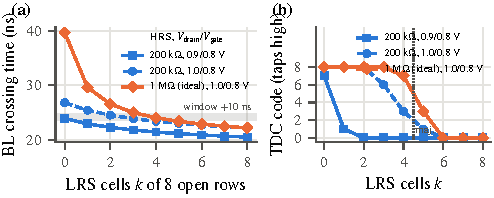
\includegraphics[width=\columnwidth]{grid}
\caption{8-row read with $k$ cells in the LRS, at 200\,k$\Omega$ and 1\,M$\Omega$ HRS: (a) bit-line crossing time, with the +10\,ns window shaded; (b) simulated TDC code.}
\label{fig:pim}
\end{figure}
Because $\Vd$ stays at or below 1\,V, the settle cycle must ground SL (the settle-drain bit of the controller), since with SL floating, charge sharing takes BL below the buffer threshold before READ.
The full supply grid was simulated for both HRS values, the codes at every window position were computed from the simulated crossing times and tap tables, and the best point of each operation was then simulated directly.
Table~\ref{tab:pim} lists these points and Fig.~\ref{fig:pim} shows the crossing times and codes behind them.

At 200\,k$\Omega$ every multi-row operation is resolved at $\Vg=0.8$\,V and at no higher word-line voltage, because the current-limited cells stretch the 8-row discharge band to 20 to 27\,ns (Fig.~\ref{fig:pim}(a)), wide enough for $\Vd$ to place it against the window grid, whereas at $\Vg\ge0.9$\,V the band is shorter than the 10\,ns offset step and falls between window positions.
At $\Vd=0.9$\,V the all-HRS crossing (23.9\,ns) lies inside the window and the $k=1$ crossing (22.9\,ns) before it, which gives the codes 7, 1, 0, \ldots\ of Fig.~\ref{fig:pim}(b) and a NOR margin of six taps, and the ideal 1\,M$\Omega$ reaches the full scale.
The majority is harder, because the step from $k$ to $k+1$ shrinks as $1/k^2$, so $c(4)-c(5)$ needs the window on the compressed part of the band; $\Vd=1.0$\,V moves it there and gives a majority by two taps, or four at 1\,M$\Omega$.
The 10\,ns step, one clock period, is thus the main limitation of the design, since it caps both the row count and the hot-corner margins that follow.

\subsection{Rows per access, corners, and temperature}
\label{sec:rows}
\begin{table}[!t]
\centering
\caption{Margin in taps vs.\ temperature at 200\,k$\Omega$, fixed / re-tuned setting}
\label{tab:retune}
\scriptsize
\setlength{\tabcolsep}{4pt}
\begin{tabular}{@{}lccc@{}}
\toprule
 & $-40$\,\si{\celsius} & 27\,\si{\celsius} & 125\,\si{\celsius}\\
\midrule
read, 1 row & 8 / 8 & 8 / 8 & 8 / 8\\
NOR, 8 rows & 0 / 5 & 5 / 5 & 0 / 1\\
majority, 8 rows & 0 / 2 & 2 / 2 & 0 / 0\\
\bottomrule
\end{tabular}
\end{table}
\begin{figure}[!t]
\centering
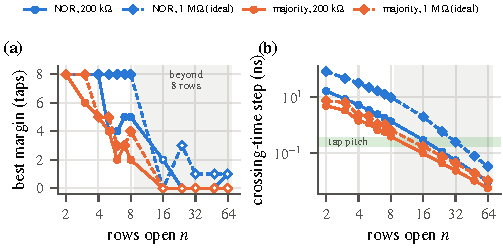
\includegraphics[width=\columnwidth]{rows}
\caption{Rows per access: (a) best NOR and majority margin; (b) crossing-time step behind each decision against the tap pitch (shaded). Hollow markers: at the best 8-row supplies.}
\label{fig:rows}
\end{figure}
Fig.~\ref{fig:rows} extends the same model from one to eight rows over the full supply grid, and to 16 to 64 rows at the best 8-row supplies.
At 200\,k$\Omega$ the NOR keeps all eight taps up to four rows and four to five taps up to eight, while the majority falls from eight taps at two rows to two or three at six to eight.
Every open row adds an HRS current against which one LRS cell must stand out, so the crossing-time step behind each decision falls roughly as $1/n^2$ (Fig.~\ref{fig:rows}(b)), from 17\,ns (NOR) and 5\,ns (majority) at two rows to 1.4 and 0.4\,ns at eight.
From 16 rows on, the step at 200\,k$\Omega$ is at or below a tap pitch, and the single-tap margins computed there are tap-edge artifacts.
One access therefore decides over at most eight rows at the characterized HRS, wider sums are split into eight-row groups that the host combines, and only two rows give a distinct code for every count.

Over the process corners and $-40$ to 125\,\si{\celsius} the 8-row band moves from 16 to 60\,ns against the 10\,ns window step, and this is where the tunability matters (Table~\ref{tab:retune}).
With the room-temperature setting held fixed, the 8-row operations are lost at both temperature extremes, whereas re-tuning $\Vd$, $\Vg$, $\Vdel$, and the offset per temperature keeps the single-row read at eight taps everywhere and recovers the 8-row NOR at $-40$\,\si{\celsius} with five taps, but not at 125\,\si{\celsius}, where the band is shorter than the step and one tap remains.

\subsection{Read disturb and the device budget}
A read biases the selected cells in the RESET polarity, with BL high and SL grounded, so repeated reads push the cells toward the HRS, and it is $\Vg$ rather than $\Vd$ that sets the stress.
At the best points a cell sees at most 0.06 to 0.12\,V and 0.8 to 1.3\,\si{\micro\ampere}, below the 0.2\,V read condition of the device and a sixth of its 8\,\si{\micro\ampere} RESET target.
On these devices $10^5$ pulses of 10\,\si{\micro\second} at 0.1 to 0.2\,V leave every level unchanged and drift starts at 0.3\,V, while retention alone lowers the LRS by 15\,\% in 100\,h at room temperature~\cite{baroni2026drift}, so the refresh interval is set by retention and temperature rather than by the read count.

The margins above hold at the typical corner with fixed resistances, and the final question is how much spread they tolerate.
With a 3 to 3.6:1 current contrast, a Monte Carlo analysis on the simulated crossing times, checked against 160 SPICE runs with drawn cell resistances, limits the HRS spread for an $n$-row decision at a $10^{-3}$ error rate to $\sigma_{\ln R}\approx0.46/\sqrt{n}$ with an ideal threshold, which is 0.46 for a single row, 0.33 for two rows, and 0.16 for eight.
Measured arrays show 0.3 to 0.6 on the 250\,nm devices and 0.5 to 1 on the Al-doped 130\,nm devices, whose HRS at the same verify has a median of 90 to 220\,k$\Omega$ but a conductive edge pinned at 50\,k$\Omega$~\cite{perez2017hfalo,baroni2025aldoping}.
The single-row read therefore works at the characterized HRS, whereas the 8-row logic needs the deeper reset of the 1\,M$\Omega$ rows of Table~\ref{tab:pim}, which buys a full-scale 8-row NOR, a four-tap majority, and an eight-row spread limit of 0.5, inside the measured range.
A deeper reset, a tighter verify window, and fewer rows per access are the levers, and a higher word-line voltage adds only 30 to 45\,\% of contrast.
The first two are programming-time costs, since a deeper reset takes more incremental-step-pulse-with-verify (ISPVA) pulses per write, about twelve of 12\,\si{\micro\second} at the 5\,\si{\micro\ampere} target~\cite{perez2017hfalo}, and with Al doping leaves a quarter of the cells at the read floor~\cite{baroni2025aldoping}, while a tighter window costs further verify iterations.

\subsection{Comparison and limitations}
\begin{table}[!t]
\centering
\caption{Comparison with RRAM and time-domain macros}
\label{tab:prior}
\scriptsize
\setlength{\tabcolsep}{1.7pt}
\begin{tabular}{@{}llllll@{}}
\toprule
 & node & memory & readout & summed$^\mathrm{a}$ & reported metric\\
\midrule
\cite{chen2018rram65nm} & 65\,nm & 1\,Mb 1T1R & current SA, 3\,b & 9--25 & 14.8\,ns/cycle\\
\cite{wan2022neurram} & 130\,nm & 3\,Mb 1T1R & ADC, calibrated & 256 & 43\,TOPS/W (1\,b)\\
\cite{sayal2020timedomain} & 40\,nm & none on chip & counter TDC & 25--150, serial & 12.1\,TOPS/W\\
\cite{xue2024tdcim} & 180\,nm & 8\,kb SRAM & counter TDC & 32 per chain & 0.3--0.8\,TOPS/W$^\mathrm{b}$\\
this work & 130\,nm & 4\,kb 1T1R & 8-tap TDC, tunable & $\le8$ & 0.13--0.2\,pJ/bit$^\mathrm{c}$\\
\bottomrule
\multicolumn{6}{@{}p{\columnwidth}@{}}{\scriptsize $^\mathrm{a}$cells sensed in one access; $^\mathrm{b}$8$\times$8\,b at 1.2\,V; $^\mathrm{c}$slice SPICE, 0.45\,\si{\micro\second} per access; SA: sense amplifier.}\\
\end{tabular}

\end{table}
Table~\ref{tab:prior} places the read next to the silicon RRAM and time-domain macros it draws on.
Those macros are MAC engines, so the table compares structure rather than figures of merit, and against their reference-tracked or calibrated readouts this work trades throughput for a bitwise read of up to eight rows whose every timing and drive level is a register or a pad.
The evaluation rests on an 8$\times$8 slice with resistor cells and a single value of $C_\mathrm{MIM}$, and its disturb bound rests on SET-polarity data, so the HRS spread and the RESET-polarity disturb are the first quantities to measure on silicon, while a fractional-cycle offset, which would lift the eight-row cap and the loss at 125\,\si{\celsius}, is the first change for a second version.

\section{Conclusion}
\label{sec:concl}
This paper set out from the observation that the read circuit of an RRAM PiM array is designed against a model that the fabricated cells do not follow, and proposed a read whose operating point is chosen after fabrication instead.
Converting the bit-line discharge time into a thermometer code puts the decision into a window that registers and supply pads can move, and opening several rows turns the same read into an in-memory NOR or majority.
Implemented in a tape-out-ready 64$\times$64 1T1R macro and simulated with the extracted loading of its bit lines, the read separates a single row by eight taps and resolves an 8-row NOR by six taps and a majority by two, and re-tuning restores these margins across temperature where a fixed setting loses them.
The same simulation yields the budget that the device has to meet, a resistance spread of 0.46 for a single row and 0.16 for eight rows at the characterized high-resistance state, or 0.5 with a deeper reset, so that spread is the first quantity to measure on silicon.


\bibliographystyle{IEEEtran}
\bibliography{refs}

\end{document}
